\subsection{Đăng ký tài khoản người dùng}
\subsubsection*{Mục tiêu}
Cho phép người dùng tạo tài khoản bằng cách điền đầy đủ thông tin cá nhân và \codefile{passphrase} (đảm bảo đủ an toàn). Thông tin sau đó được kiểm tra tính hợp lệ, hash \codefile{passphrase} và lưu vào cơ sở dữ liệu. Đồng thời tạo \codefile{recovery key} và cung cấp cho người dùng.

\subsubsection*{Giao diện}
Giao diện \codefile{/auth/signup} là form HTML bao gồm các trường:
\begin{itemize}
    \item Email
    \item Họ tên
    \item Ngày sinh
    \item Số điện thoại
    \item Địa chỉ
    \item Passphrase và xác nhận passphrase
\end{itemize}
\begin{figure}[H]
\centering
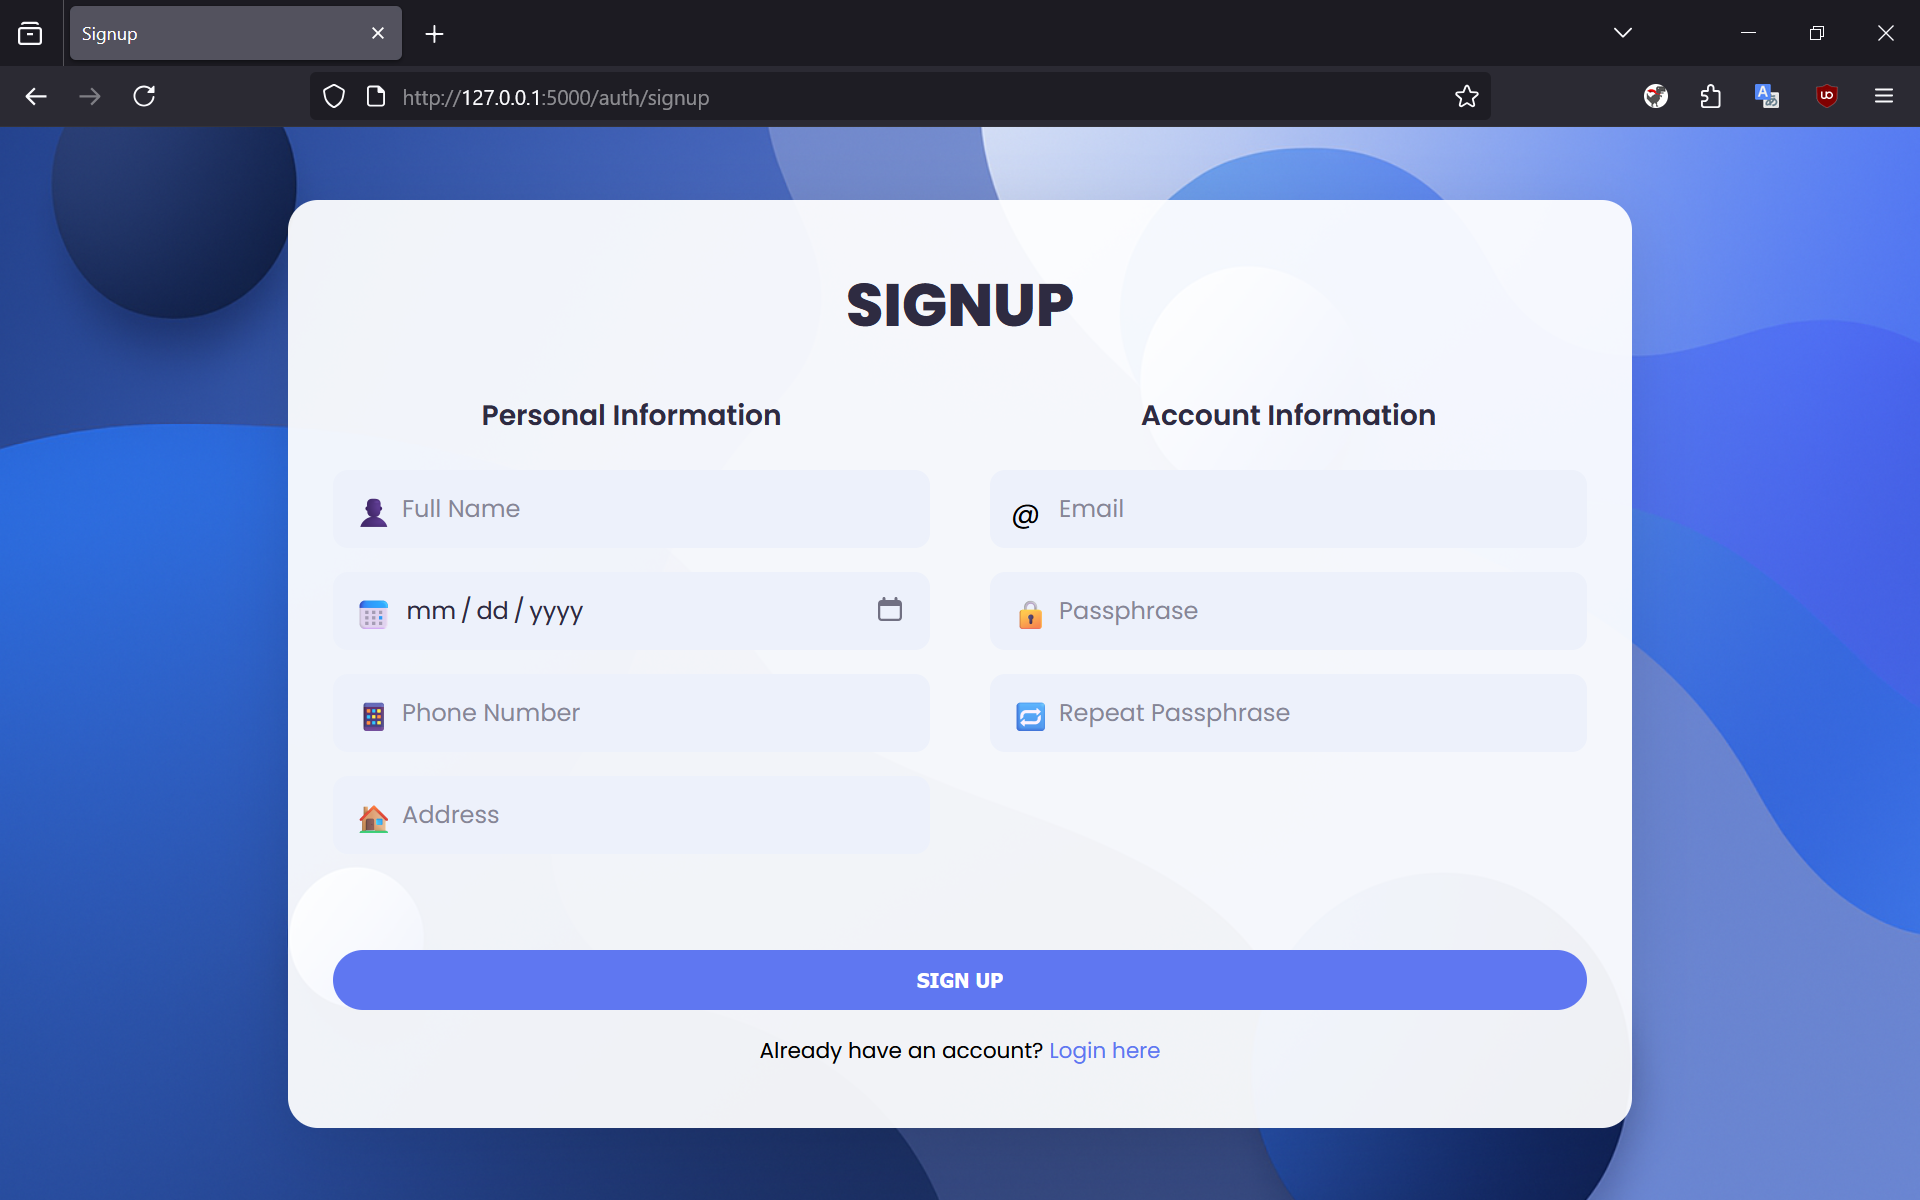
\includegraphics[scale=0.34]{img/sign-up.png}
\caption{Giao diện Signup}
\label{fig:signup_ui}
\end{figure}

Khi đăng ký thành công, hệ thống sẽ hiển thị mã khôi phục tài khoản, yêu cầu người dùng lưu lại mã này để phục hồi nếu mất mật khẩu.
\begin{figure}[H]
\centering
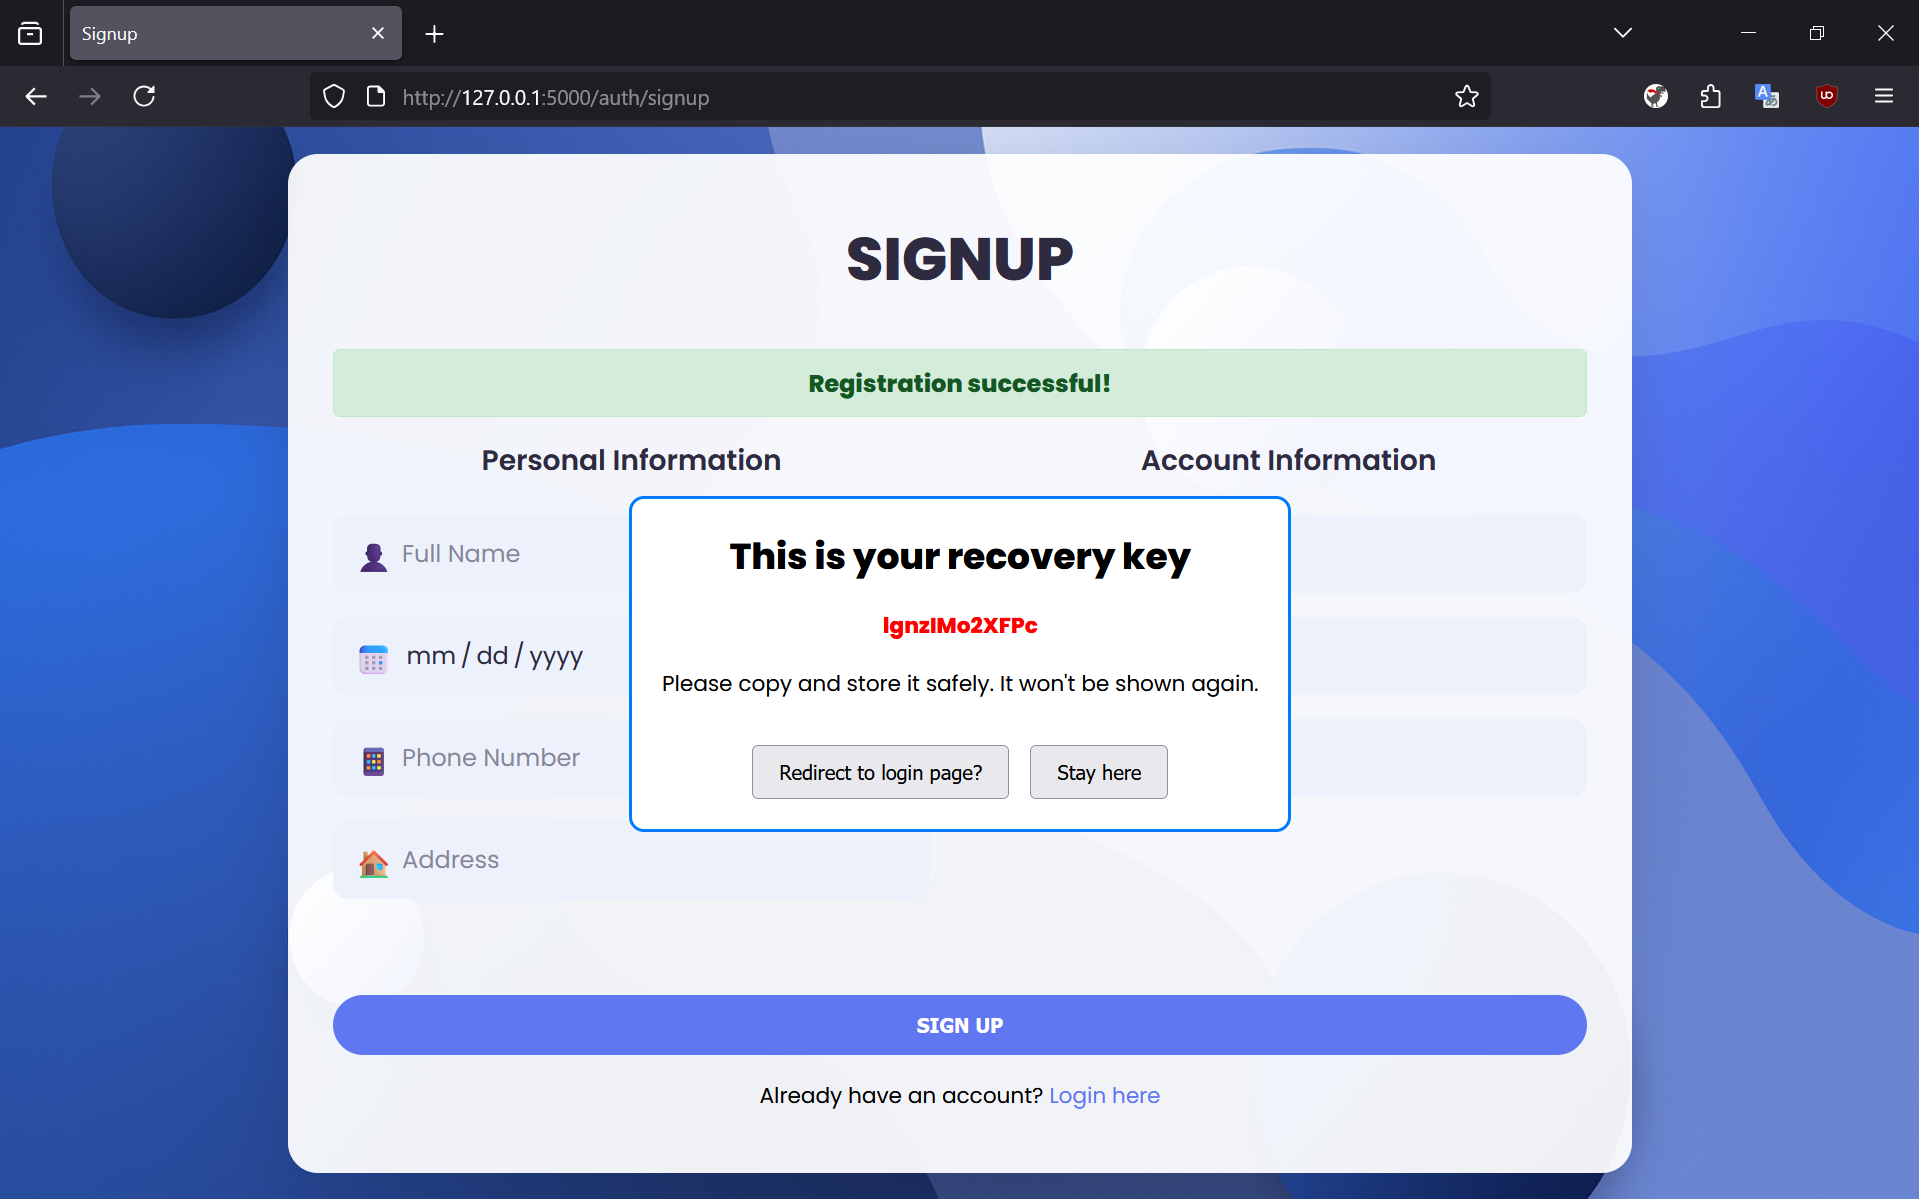
\includegraphics[scale=0.34]{img/recovery-key.png}
\caption{Giao diện popup recovery key}
\label{fig:recovery_key_ui}
\end{figure}

\subsubsection*{Quy trình thực hiện}
\begin{enumerate}
    \item Người dùng nhập thông tin và submit form $\rightarrow$ POST \codefile{/signup}
    \item Flask gọi hàm \codefile{register\_user(request.form)} trong \codefile{logic.py}
    \item Thông tin được kiểm tra và chuẩn hóa:
    \begin{itemize}
        \item Email hợp lệ (\codefile{is\_valid\_email})
        \item Ngày sinh đúng định dạng (\codefile{is\_valid\_date})
        \item Số điện thoại gồm đúng 10 chữ số (\codefile{is\_valid\_phone}) 
        \item Passphrase đủ mạnh (\codefile{is\_strong\_passphrase})
    \end{itemize}
    \item Nếu hợp lệ:
    \begin{itemize}
        \item Sinh \codefile{salt} ngẫu nhiên
        \item Băm \codefile{passphrase} kết hợp với salt bằng \codefile{SHA-256}
        \item Sinh \codefile{recovery\_code} để dùng cho khôi phục
        \item Sinh \codefile{mfa\_secret} phục vụ TOTP trong MFA
    \end{itemize}
    \item Thực hiện \codefile{INSERT} bản ghi vào bảng \codefile{users} trong CSDL
    \item Ghi log hành động: \codefile{log\_user\_action(email, "Register", "Success")}
    \item Trả về kết quả thành công và hiển thị mã khôi phục
\end{enumerate}

\subsubsection*{Chi tiết kỹ thuật và thư viện bảo mật}
\textbf{1. Hashing passphrase với Salt}

Thư viện: \codefile{hashlib, os} 

Kỹ thuật:
\begin{itemize}
    \item Salt được sinh bằng \codefile{os.urandom(16).hex()} $\rightarrow$ đảm bảo tính ngẫu nhiên mạnh.
    \item \codefile{passphrase} được hash bằng \codefile{SHA-256(passphrase + salt)} trước khi lưu xuống DB.
\end{itemize}

\textbf{2.Validator kiểm tra đầu vào}

Thư viện: \codefile{re, datetime} 

Kỹ thuật:
\begin{itemize}
    \item Regex kiểm tra định dạng email, số điện thoại.
    \item Kiểm tra \codefile{passphrase} phải ít nhất 8 ký tự, chứa chữ hoa, số, ký hiệu.
    \item Loại bỏ ký tự nguy hiểm khỏi input (\codefile{sanitize\_input()}) $\rightarrow$ giảm rủi ro XSS / SQLi / Code Injection.
\end{itemize}

\textbf{3. Tạo mã khôi phục}

Thư viện: \codefile{random, string} 

Kỹ thuật:
\begin{itemize}
    \item Sinh chuỗi ngẫu nhiên gồm chữ + số, dùng 1 lần.
    \item Người dùng được yêu cầu lưu lại $\rightarrow$ dùng khi mất \codefile{passphrase}.
    \item Được lưu trong DB (\codefile{users.recovery\_code}) và xóa sau khi reset thành công.
\end{itemize}

